V aplikaci se nachází tři skupiny presnterů, podle příslušnosti k modulu: Core, Backend a Frontend. Šablony pro konkrétní Presenter jsou ve společném adresáři \tt{templates/jmenoPresenteru/} a název souboru každé šablony odpovídá akci daného presenteru. Pokud akce nevede na vykreslení šablony, nemusí mít šablonu vůbec vytvořenou. Příkladem je \tt{Sign:out} (\it{SignPresenter} a akce \it{out}), která přihlášeného uživatele odhlásí a přesměruje na přihlašovací formulář \tt{Sign:in} (stejný presenter, akce \textit{In}). SignPresenter obsahuje metodu \phpinline{renderIn} a tedy vyžaduje i šablonu \tt{templates/Sign/in.latte}

%--------------%
%--------------%

\n{3}{Frontend}

%--------------%
\begin{figure}[h]
	\centering
	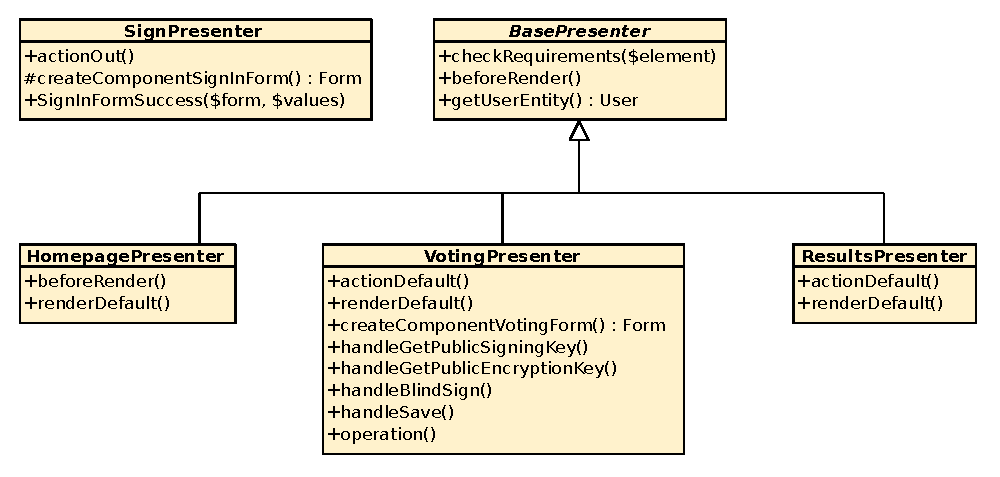
\includegraphics[width=\linewidth]{svg/frontendPresenters.eps}
	\captionsetup{width=\linewidth}
	\caption[Třídy Presenter frontendové části]{Třídy Presenter frontendové části (zdroj: vlastní)}
	\label{fig:FrontendPresenters}
\end{figure}
\clearpage
\paragraph{SignPresenter} Jediným úkolem tohoto presenteru je uživateli poskytnout možnosti přihlášení a odhlášení.

% \tab{popisek}{label}{rozměr (0.0 - 1.0)}{definice sloupců}{obsah} 
\tab{Dostupné akce}{tab:FrontendSignPresenterAction}{1}{c|ccc}{
	\hline
	akce & action* & render* & šablona \\
	\hline
	in & - & - & in.latte \\
	out & actionOut & - & - \\
}
Dostupné akce:
\begin{itemize}
	\item \tt{Sign:in} Zobrazí přihlašovací formulář\\
Nemá definované metody action ani render - ekvivalentní by byly prázdné metody. Jediným úkolem této metody je zobrazit formulář pro přihlášení, který se vytváří metodou \phpinline{SignPresenter::createComponentSignInForm()}. Po~odeslání formuláře se volá opět tato akce, nicméně se provede i callback formuláře \phpinline{SignPresenter::signInFormSuccess()}. V tomto callbacku se aplikace pokusí o přihlášení uživatele pomocí poskytnutých údajů. Presenter je předá třídě implementující rozhraní \phpinline{Nette\Security\IAuthenticator}. Princip přihlašování je popsán v části \ref{section:prihlasovani}. Na tuto akci zároveň odkazují všichni potomci BasePresenter z metody \phpinline{BasePresenter::checkRequirements()}, pokud se uživatel pokusí provést jakoukoli akci jako nepřihlášený (např. po~vypršení session).
	\item \tt{Sign:out} Odhlásí uživatele\\
Uživatel po kliknutí na odkaz ,,Odhlásit'' vyvolá akci tuto akci, kdy je odhlášen a následně přesměrován na přihlašovací formulář -- \tt{Sign:in}. Tato akce nemá render metodu ani šablonu (dochází k přesměrování, které předchází jakémukoli výstupu a ukončuje aktuální cyklus aplikace).
\end{itemize}


%--------------%
\paragraph{BasePresenter} je abstraktní třída, která je společným předkem pro všechny presentery, které jsou dostupné pouze po přihlášení. Také obsahuje metody, které jsou užitečné pro všechny presentery obecně. Vzhledem k tomu, že se jedná o abstraktní presenter, nemá žádné metody action, render ani vlastní šablony. 
Metoda \phpinline{checkRequirements()} slouží k ověření, že je uživatel přihlášen. Rozšiřuje rodičovskou metodu, která detekuje CSRF\footnote{Cross-Site Request Forgery} útoky, je tedy nezbytné zahrnout \phpinline{parent::checkRequirements($element)}%$
. Aby bylo zajištěno správné zobrazení krátkých stavových zpráv \it{flashMessage} a modálních oken během AJAX požadavků, je zde i metoda \phpinline{beforeRender()}, která se volá vždy před metodami \phpinline{render}.


%--------------%
\paragraph{HomePagePresenter} slouží jako rozcestník po přihlášení uživatele. Jeho jediná akce je \texttt{Homepage:default}, a obsahuje pouze render metodu, která získává objekty Election, které jsou dostupné danému uživateli.


%--------------%
\paragraph{VotingPresenter} je stěžejním presenterem frontendové části aplikace, jejímž prostřednictvím probíhá celý proces volby na straně uživatele. Metoda \phpinline{actionDefault()} získává a \phpinline{renderDefault()}  předává šabloně objekt \phpinline{Election}. Samotný hlasovací lístek je tvořen formulářem. Ten je vytvářen tovární metodou \phpinline{createComponentVotingForm()}. Zde bylo využito \it{generované továrničky}, což je zjednodušený zápis továrních tříd, které pouze vytváří jeden konkrétní objekt. Do~presenteru je pomocí Dependency Injection předána závislost na rozhraní \phpinline{VotingFormFactory} a Nette samo vygeneruje implementaci tohoto rozhraní, které je předáno do Presenteru \cite{Planette}.

Formulář \phpinline{VotingForm} je samostatnou třídou rošiřující \phpinline{Control}\footnote{\Verb{Nette\Application\UI\Control}} - v názvosloví Nette komponentou. Komponenty mohou mít vlastní šablony, což umžňuje zpřehlednit šablonu presenteru pokud není celý formulář vykreslován automaticky přes \phpinline{FormRenderer}. Zároveň je i samotný kód presenteru jednodušší, o vytvoření formuláře, validaci a zpracování se totiž stará třída formuláře.

Hlasovací formulář neobsahuje žádnou logiku pro validaci ani zpracování odeslaných dat. Veškerá validace probíhá pomocí JavaScriptu na straně klienta a data se odesílají teprve po zašifrování a to přímo na presenter pomocí AJAX. Zpracování těchto požadavků (signálů) pomocí handle metod je popsáno v samostatné části~\ref{section:zpracovaniHlasu}~věnované zpracování hlasovacích lístků.


%--------------%
\paragraph{ResultsPresenter} je velice jednoduchý presenter, který opět pomocí metod \phpinline{actionDefault()} a \phpinline{renderDefault()} získá a zpřístupní objekt \phpinline{Election} šabloně k~zobrazení výsledků hlasování / voleb.



%--------------%
%--------------%
\n{3}{Backend}


Tato část obsahuje nástroje pro správu uživatelů, uživatelských oprávnění a~především voleb samotných. Je hojně využíváno formulářů a interaktivních tabulek (neboli datagridů). Formuláře a datagridy jsou samostatné komponenty\footnote{třídy rozšiřující \phpinline{Nette\Application\UI\Control}}. Jednoduché komponenty jsou zpravidla vytvářeny přímo v Presenteru. Složitější chování nebo obsáhlé komponenty je vhodnější oddělit do samostatné třídy. Podrobněji jsou datagridy popsány v části \ref{section:Datagridy}.

\begin{figure}[h]
	\centering
	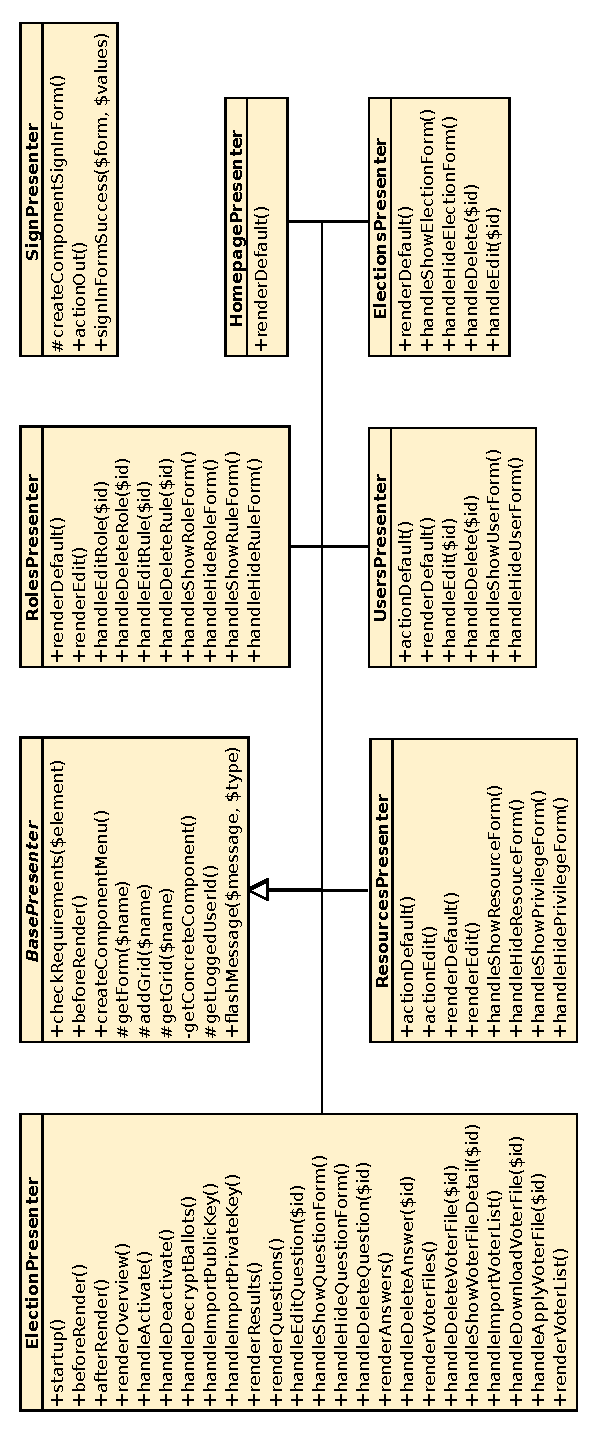
\includegraphics[height=\textheight]{svg/backendPresentersPortrait.eps}
	\captionsetup{width=\linewidth}
	\caption[Třídy Presenter backendové části]{Třídy Presenter backendové části (zdroj: vlastní)}
	\label{fig:BackendPresenters}
\end{figure}
\clearpage

%--------------%
\paragraph{SignPresenter} slouží ke správě přihlášení do aplikace, v zásadě se jedná o obdobu frontendového \phpinline{SignPresenter}. Popis této třídy je tedy identický.


%--------------%
\paragraph{BasePresenter} je stejně jako \phpinline{App\Frontend\Presenters\BasePresenter} abstraktní třídou společnou pro všechny další presentery. Ověřuje, že uživatel je přihlášen a má oprávnění provést požadovanou akci.


%--------------%
\paragraph{HomepagePresenter} hlavní jeho funkcí je umožnit zobrazení navigace po přihlášení i pro uživatele, který nemá definovaná žádná práva a jediné co může v aplikaci provést je se odhlásit. Mohl by zobrazovat i nějakou formu rozcestníku, jako ve frontendové části, to ale obstarává navigační lišta. Dalším vhodným využitím tohoto presenteru by byla prezentace důležitých dat formou \it{dashboardu}.


%--------------%
\paragraph{ElectionsPresenter} poskytuje přehled nad všemi vypsanými volbami, jejich rychlou editaci, mazání a odkaz na zobrazení detailu. Nové volby se také vytváří v tomto presenteru. Při vypisování nových voleb je vhodné zvolit výstižný krátký popisek, jeho editace je uživatelsky přívětivá díky JavaScriptovému pluginu \it{tinyMCE}.


%--------------%
\paragraph{ElectionPresenter} nabízí detailní přehled konkrétních voleb rozdělený do záložek. Některé záložky se zobrazují pouze pokud se volby nacházejí v určitém stavu. Záložka výsledky se například zobrazí až po ukončení voleb. 

V záhlaví detailu se nachází kontextové menu, které umožňuje volby (de)aktivovat, nahrávat seznamy voličů a klíče volební komise. Aktivace voleb způsobí jejich zobrazení voličům, hlasování je umožněno až v řádném termínu. Po aktivaci voleb není možné měnit jejich nastavení, ale lze je opět deaktivovat. Aktivovat a deaktivovat volby lze pouze pokud se nenacházejí v průběhu jejich konání. Po skončení voleb se voličům ukazují pouze výsledky a to do doby než jsou deaktivovány.

Jednotlivými záložkami jsou:
\begin{itemize}
	\item \b{Overview}, kde se zobrazuje formátovaný popis voleb a tři pole s šifrovacími klíči (pokud jsou dostupné). Těmito klíči jsou: privátní a veřejný klíč volební komise a veřejný podpisový klíč serveru.
	\item \b{Results} s výsledky voleb. Tato záložka je distupná pouze po ukončení voleb. V~případě, že dosud nejsou spočítané výsledky, je nabídnuto jejich spočítání a~následně se již zobrazují pouze výsledky v přehledných grafech.
	\item \b{Questions} zobrazí grid otázek definovaných pro dané volby. Otázkou může být volená pozice, její odpověďmi pak jména kandidátů. Při založení nové otázky je možné nastavit minimální a maximální počet otázek, zda je odpověď povinná a~jednotlivé odpovědi. V gridu je možné otázky editovat a mazat.
	
	\item \b{Answers} obsahuje grid všech odpovědí, které byly definované při zakládání otázek, zde je možné odpovědi mazat.
	
	\item \b{Voter list} zobrazí grid s aktivním seznamem voličů.
	
	\item \b{Voter files} v tomto gridu se nachází všechny soubory se seznamem voličů, které byly pro dané volby nahrány. Soubory je možno prohlížet, mazat, stáhnout a~aplikovat vybraný soubor jako aktivní seznam voličů. Nový soubor lze nahrát přes kontextové menu v záhlaví.
	
\end{itemize}


%--------------%
\paragraph{UsersPresenter} jednoduchý presenter s gridem uživatelů a formulářem pro přidávání / editaci uživatelů. Formulář umožňuje uživatelům přidělovat role i změnit heslo. Aplikace neobsahuje žádný registrační formulář, nové uživatele musí vždy přidávat osoba s patřičným oprávněním - pravděpodobně administrátor aplikace. Jak bylo popsáno v části \ref{section:prihlasovani}, není potřeba zakládat uživatelské účty voličům, ale pouze osobám, kterým je potřeba navýšit oprávnění.

%--------------%
\paragraph{RolesPresenter} výchozí View tohoto presenteru nabízí grid všech dostupných rolí a~formulář pro jejich základní editaci. Pomocí akce gridu je možné zobrazit detail role, kde se nachází seznam definovaných pravidel přístupu ve formě gridu. Tato pravidla lze editovat, mazat a přidávat nová.

%--------------%
\paragraph{ResourcesPresenter} velice podobý předchozímu RolePresenter. Tento umožňuje správu prostředků (\textit{Resource}), na stránce detailu je pak k dispozici správa akcí (\textit{Privilege}) dostupných pro daný prostředek.

\n{3}{Core}
Tento modul je společný pro frontendovou i backendovou část a obsahuje pouze uživatelsky přívětivé zpracování chybových stavů. Pokud se uživatel pokouší přistoupit na neexistující stránku, není nalezen požadovaný záznam v databázi (HTTP~404) nebo nemá uživatel potřebná oprávnění k zobrazení stránky (HTTP~403), místo základních chybových stránek HTTP serveru mu je zobrazena chybová stránka vygenerovaná Nette. Stejně tak v případě chyby serveru (HTTP~500). 

V případě, že se Nette nachází ve vývojovém režimu, jsou všechny chyby aplikace předávány ke zpracování nástroji Tracy (dříve Laděnka) \cite{Tracy}, který vypíše chybu včetně části zdrojového kódu, předávaných proměnných, dotazů na databázi a dalších velice užitečných informací pro ladění chyb. V produkčním režimu jsou chyby předávány \texttt{ErrorPresenteru}, který chyby 4xx předává dále do \texttt{Error4xxPresenter} případně rovnou předá statickou šablonu s chybou 500 nebo 503.

